\label{chap.3}
\section{Proposed Work}

The proposed system is an offline pipeline of five stages wrapped by an agent (Figure~\ref{fig:overview}):

\begin{enumerate}
  \item \textbf{Staging.} A compact student network, built by knowledge distillation, labels every 30-s epoch from
  EEG + EOG.
  \item \textbf{Evidence packet.} Calibrated probabilities, reliability tiers, derived metrics and a
  night-confidence tier become one versioned JSON document.
  \item \textbf{Report.} A fine-tuned small language model, run locally under a grammar, writes claims; each claim
  must cite a packet field.
  \item \textbf{Release gate.} A frozen deterministic verifier checks every claim against the packet. Only a passing
  report is rendered.
  \item \textbf{Delivery.} Exactly one page per night: a verified report, a fallback summary, a review notice or a
  rejection.
\end{enumerate}

The \textbf{agent} around them decides \emph{what to do} (quality control, finding the night, routing, retries,
resume, audit), never \emph{what is true}: stages come from the staging model, numbers from the packet, and every
sentence must pass the verifier. This restates the problem of Section~\ref{sec:problem} as a design rule: the language model is
never trusted, it is checked.

\textbf{Novelty.} The work joins compact staging and LLM reporting through an explicit contract and moves the safety
check from after release to before it. It also shows, with a mechanism, when distillation helps.

\begin{figure}[htbp]
\centering
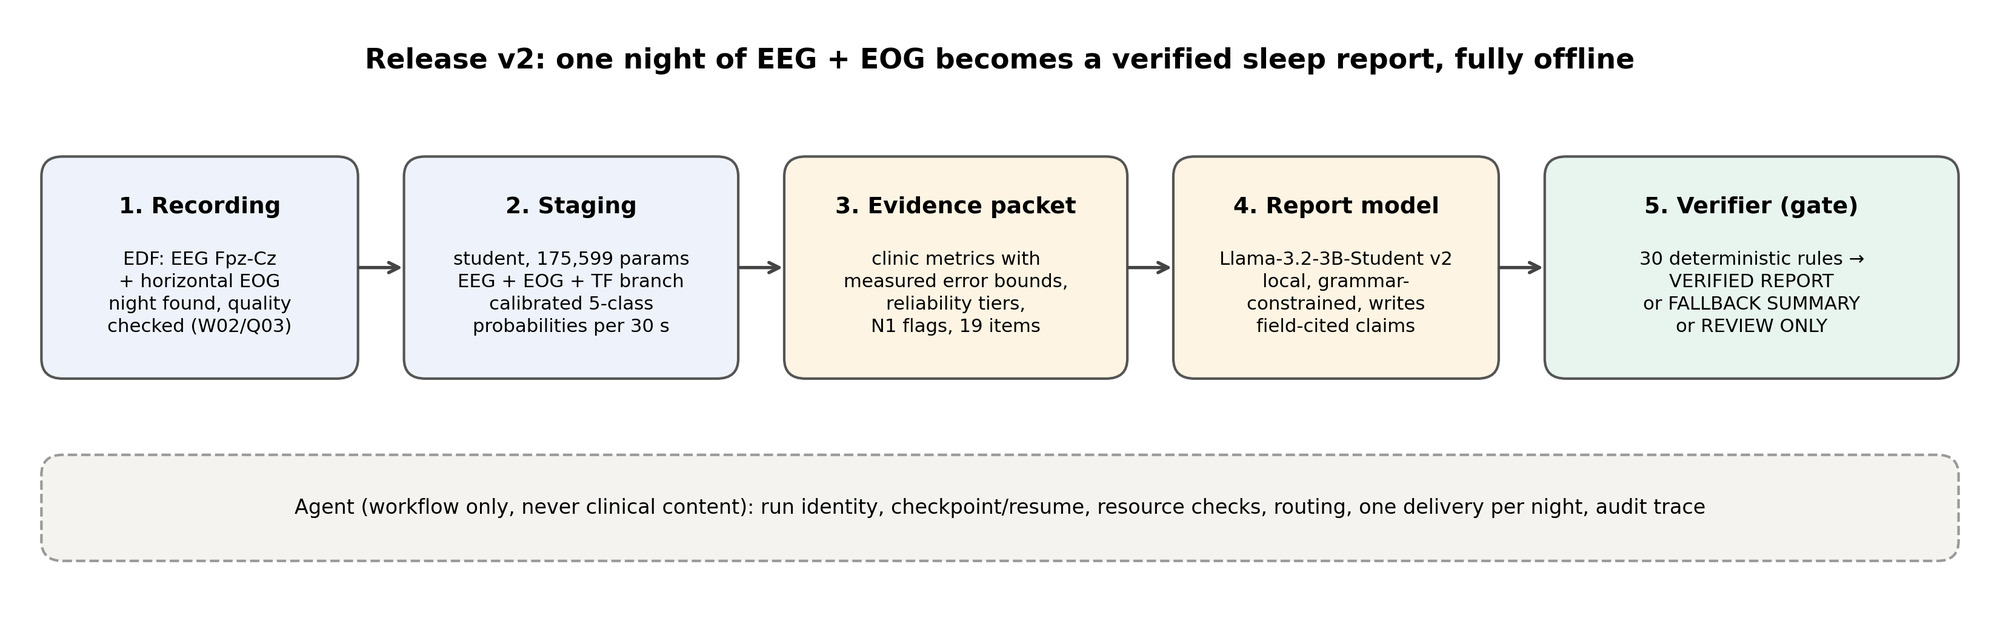
\includegraphics[width=\textwidth]{F33_system_overview.jpg}
\caption{System overview: one night of EEG + EOG becomes a verified sleep report, fully offline (release v2).}
\label{fig:overview}
\end{figure}

\subsection{ Objectives of the Proposed Work}

\begin{table}[htbp]
\centering\small
\caption{Measurable objectives.}
\label{tab:objectives}
\begin{tabularx}{\textwidth}{lYYl}
\toprule
\# & Objective & Measure & Target \\
\midrule
O1 & Leak-free staging evaluation & Subject-disjoint splits, checked in code & No subject in two splits \\
O2 & Compact, accurate student & Parameters; held-out $\kappa$ & $<$200\,K; $\ge$ teacher's $\kappa$ \\
O3 & Verified reports & Flawed reports released on the locked test set & 0 \\
O4 & Report completeness & Dev nights at 5/5 mandatory items & $\ge$25/31 (pre-registered) \\
O5 & Robust agent & Fault scenarios reaching the expected outcome & All \\
O6 & Edge readiness & Offline container: network off, no secrets, staging and report parity, ARM64 staging parity (emulated) & All met (container level) \\
\bottomrule
\end{tabularx}
\end{table}

\textbf{Secondary objectives:} calibrated confidence; measured reliability of each derived metric; byte-identical
reruns; graceful behaviour without the EOG channel; an edge budget within a Raspberry Pi 5's 16\,GB; a
plain-language summary for non-experts that only uses values the packet rates as reliable.

\section{ Methodology}

\subsection{Overview of the Approach:}

The work proceeded in six stages, each gated by a measured result before the next began (Figure~\ref{fig:pipeline}):

\begin{enumerate}
  \item \textbf{Knowledge distillation.} Audit the inherited model, rebuild subject-level splits, retrain the
  teacher, diagnose why naive KD failed, then fix the encoder and distil from an ensemble.
  \item \textbf{Student model.} Add an EOG branch, a time-frequency branch and local epoch context through gates
  that start closed; correct the labels; distil from the ensemble teacher (release v2).
  \item \textbf{Evidence packet.} Calibrate, decode the hypnogram, measure the error of every derived metric, fit
  the night-confidence tiers and the N1 flag on validation, and assemble the packet.
  \item \textbf{SLM.} Establish that the 30-rule contract is satisfiable with a large reference model, generate
  training targets, LoRA-tune small models, select on dev, evaluate once on test.
  \item \textbf{Agentic workflow.} Wrap the frozen pipeline in a deterministic state machine with quality checks,
  fallbacks and crash recovery; evaluate it with fault scenarios and invariants.
  \item \textbf{Edge simulation.} Budget time and memory analytically for a Raspberry Pi 5, then climb a simulation
  ladder (container limits, ARM64 emulation, fault replay, hardware) against pre-registered acceptance bars.
\end{enumerate}

\begin{figure}[htbp]
\centering
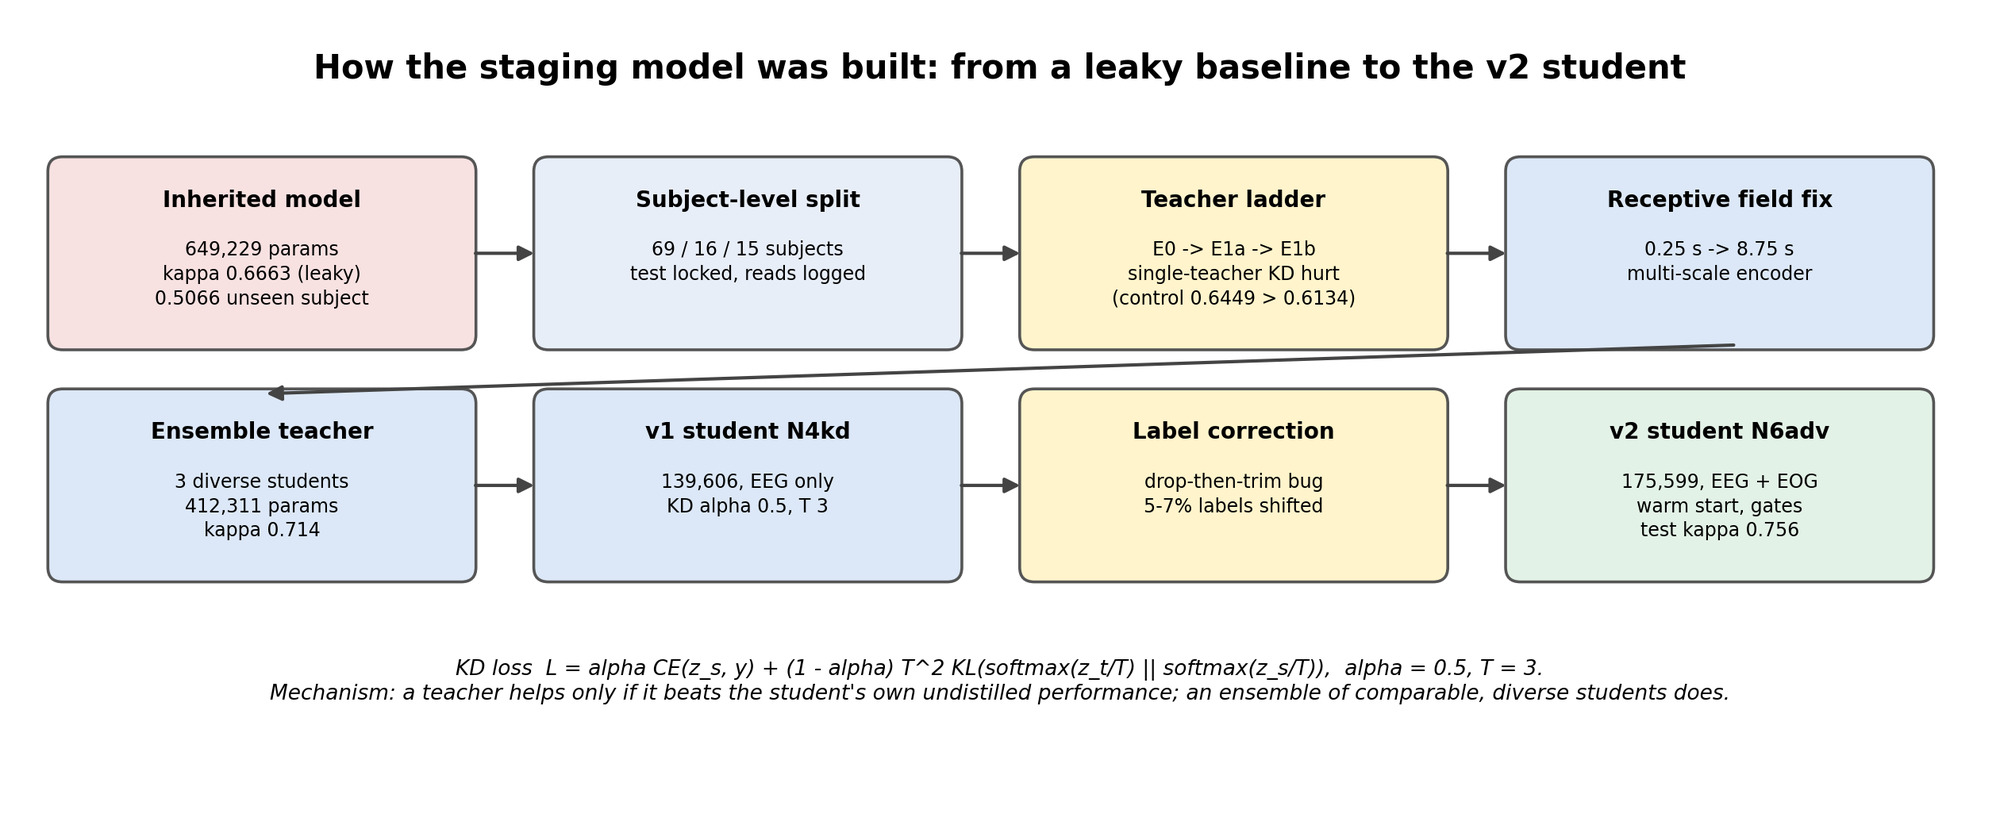
\includegraphics[width=\textwidth]{A5_training_pipeline.jpg}
\caption{How the staging model was built, from the leaky inherited baseline to the v2 student.}
\label{fig:pipeline}
\end{figure}

\subsection{Dataset Selection:}\label{sec:dataset}

\textbf{Sleep-EDFx} (PhysioNet)~\cite{kemp2000sleepedf,goldberger2000physionet}: 197 recordings (153 SC + 44 ST)
from 100 subjects; 237,950 scored epochs. Each epoch has 3,000 EEG samples (Fpz-Cz, 100\,Hz) and 34 spectral
features: for each of the six db4 wavelet sub-bands (5 levels) its energy, log-energy, entropy and variance (24), plus
STFT relative band powers (delta, theta, alpha, beta, gamma), spectral entropy, 95\% spectral edge frequency and three
band ratios (10). Release v2 adds the horizontal EOG and 8 EOG features per epoch: four band log-powers (0.3--8\,Hz),
log-variance, saccade rate, mean absolute derivative and the EOG--EEG correlation. Class shares: N2 37.4\%, W 29.5\%, REM 14.4\%, N1 10.6\%, N3 8.2\%.

Almost every subject was recorded on two consecutive nights, so a recording-level split puts the same person in
training and test. All splits are made \textbf{by subject} (first five characters of the recording ID), stratified
by cohort, and checked in code (Table~\ref{tab:splits}, Figure~\ref{fig:split}).

\begin{table}[htbp]
\centering\small
\caption{Dataset and split summary.}
\label{tab:splits}
\begin{tabularx}{\textwidth}{lrrrrY}
\toprule
Split & Subjects & Recordings & SC subj. & ST subj. & Role \\
\midrule
Train & 69 & 137 & 54 & 15 & Staging and SLM training (123 + 14 nights for the SLM) \\
Validation (dev) & 16 & 31 & 12 & 4 & Calibration, tier fitting, model selection \\
\textbf{Test (locked)} & \textbf{15} & \textbf{29} & 12 & 3 & One logged evaluation per model \\
5-fold CV & 85 & 168 & -- & -- & Architecture ablation (non-test subjects) \\
B1 benchmark & 78 & 153 & 78 & -- & Standard 10-fold subject-wise protocol \\
\bottomrule
\end{tabularx}
\end{table}

\begin{figure}[htbp]
\centering
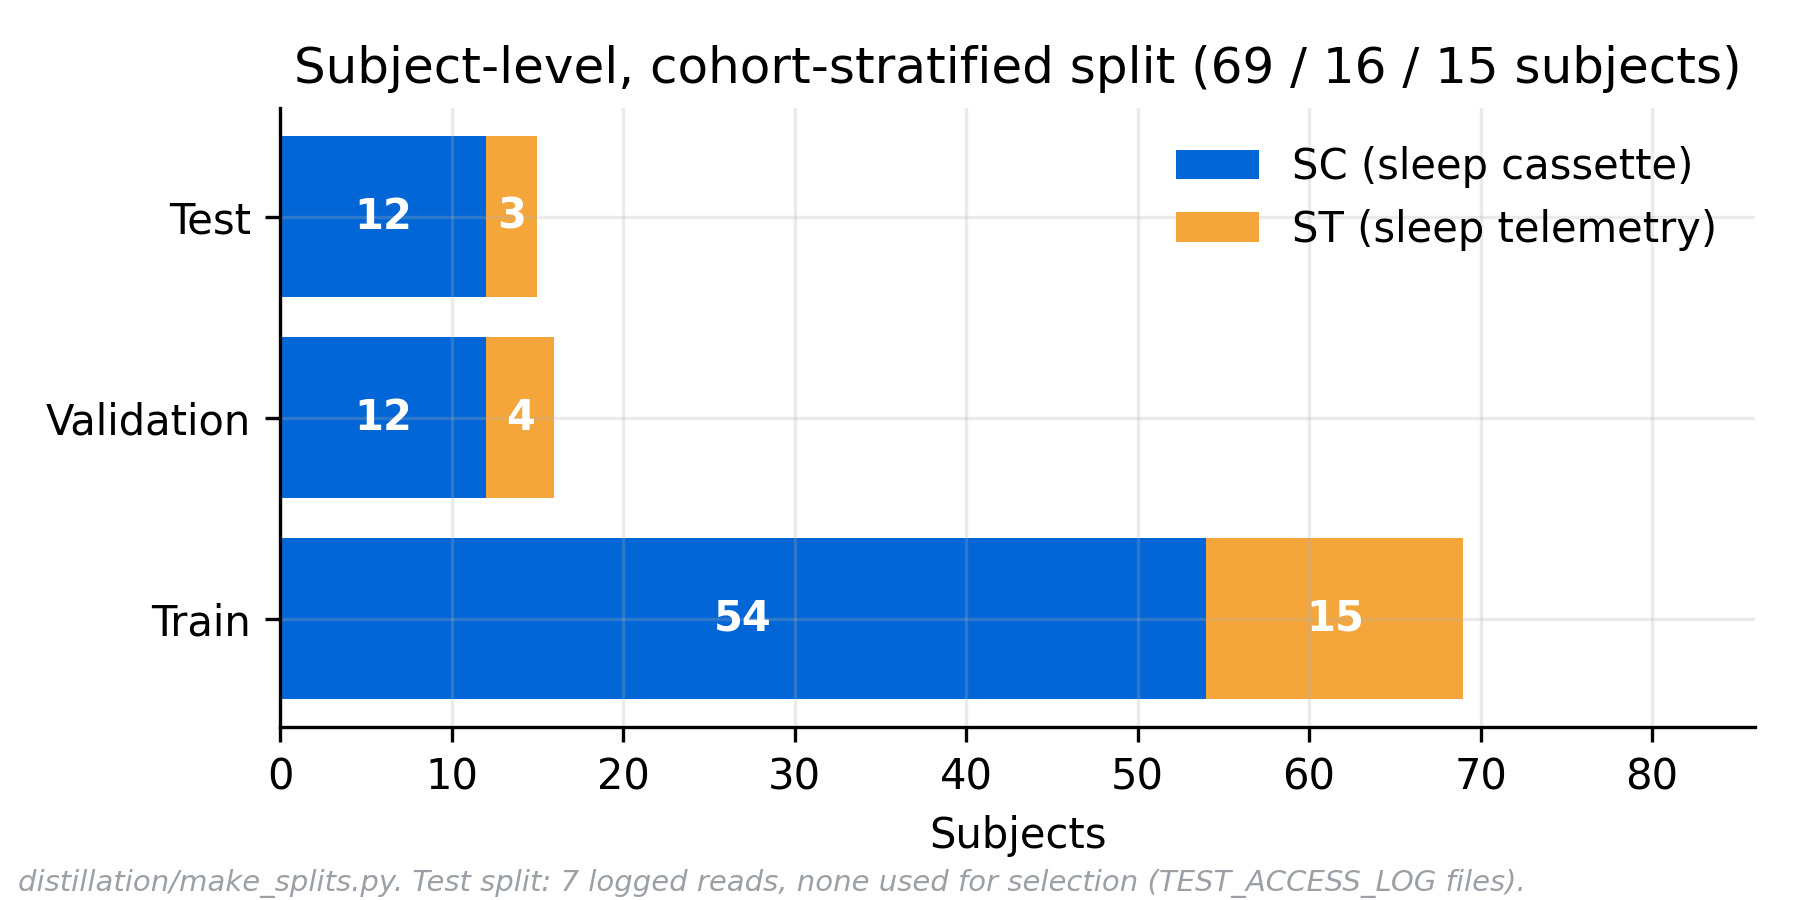
\includegraphics[width=0.85\textwidth]{F1_subject_split.jpg}
\caption{Subject-level split. Every read of the test labels is logged; none was used for selection.}
\label{fig:split}
\end{figure}

\textbf{Label correction.} The original preprocessing removed unscored epochs from the label sequence \emph{before}
computing trim points, then cut the full signal with those points, so each dropped epoch shifted every later label
by one epoch. Rebuilt from the raw hypnograms, the corrected labels change 5.65\% of training labels, 7.10\% of
validation and 5.17\% of test. \textbf{All release v2 numbers use corrected labels.} v1-era numbers in
Section~\ref{sec:res-kd} use the original \emph{stored} labels and are not comparable with v2's.

\textbf{Plain-language reference data.} For the non-expert summary, age-specific reference ranges were taken from
the National Sleep Foundation consensus~\cite{ohayon2017nsf}, Watson et al.~\cite{watson2015} and Ohayon et
al.~\cite{ohayon2004meta}, together with each subject's age, sex and cohort from the Sleep-EDF metadata.

\subsection{Algorithm/Model Design:}

\textbf{System architecture.} Figure~\ref{fig:arch} shows the three layers of the system. \emph{Offline}, run once on
a Kaggle T4 GPU, the data are split and corrected, the staging model is distilled, the packet tables are fitted on
validation and the report model is fine-tuned. Their products become the \emph{release}: a YAML file
(\texttt{agentic/config/releases/v2.yaml}) that names every file the system runs and pins it by sha256 (execution
manifest \texttt{4973f498\ldots}). At \emph{runtime}, on the device, the agent walks a raw EDF through ingest and
quality control, preprocessing, two-pass staging, packet building, report generation, the verifier and delivery,
loading each pinned file at the step that uses it. Swapping a model means writing a new release file, not new agent
code.

\begin{figure}[htbp]
\centering
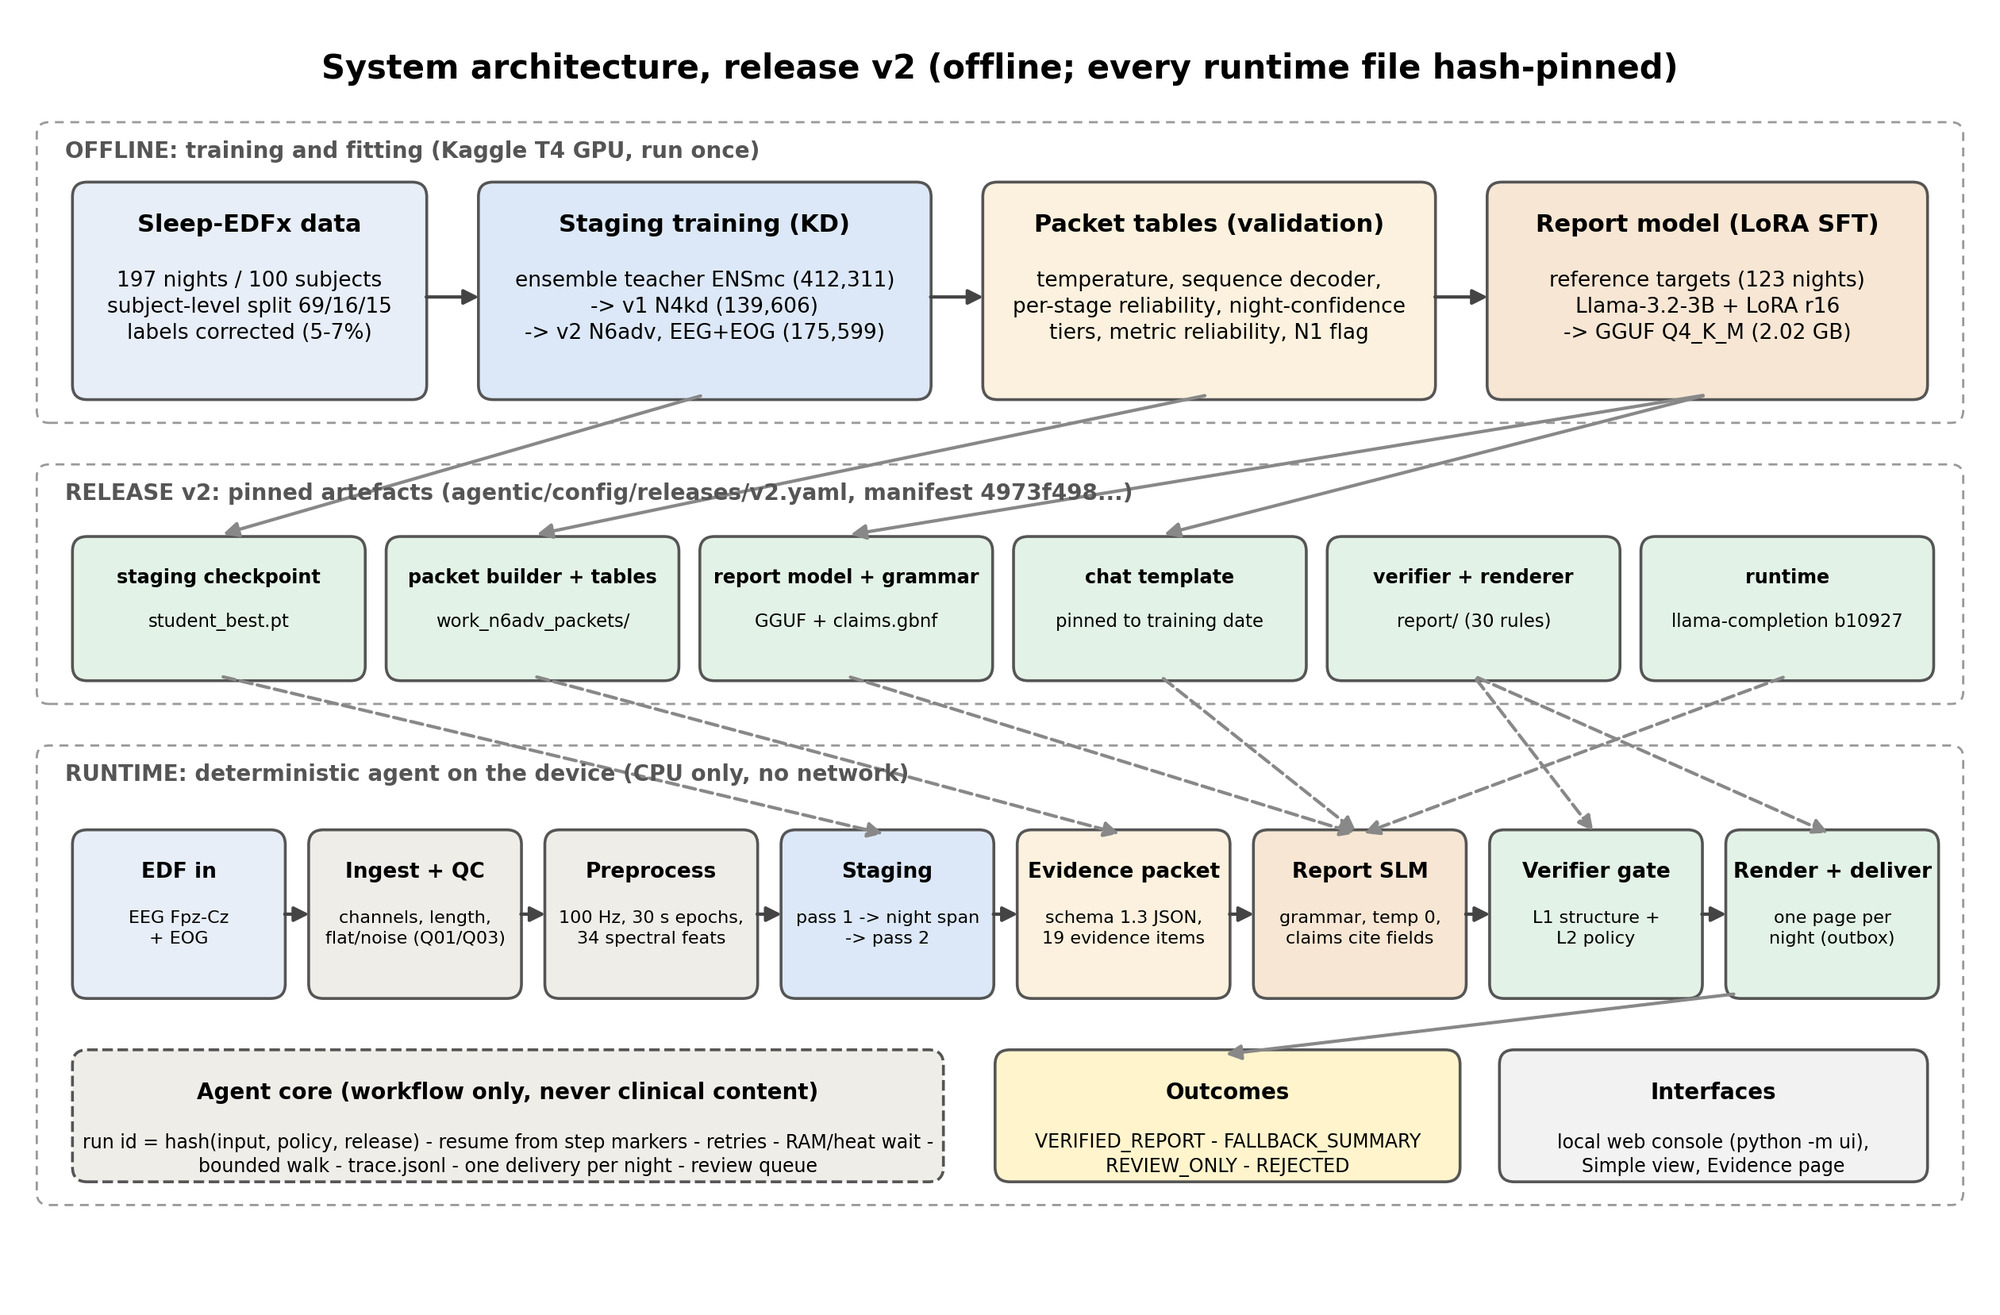
\includegraphics[width=\textwidth]{A1_system_architecture.jpg}
\caption{System architecture of release v2: offline training, the hash-pinned release, and the runtime agent pipeline.}
\label{fig:arch}
\end{figure}

\textbf{Block-wise view.} Figure~\ref{fig:blockwise} opens the same system block by block, from the input tensors to
the delivered page: (1) inputs and the 34 + 8 per-epoch features; (2) the gated multi-branch encoder with its
parameter budget against the teacher's; (3) the Transformer sequence model; (4) the distillation objective and its
result; (5) the evidence packet, the only thing downstream modules may read; (6) the report model and the two-layer
verifier; (7) the agent, delivery and the edge target. Each block also carries its measured headline result.

\begin{figure}[p]
\centering
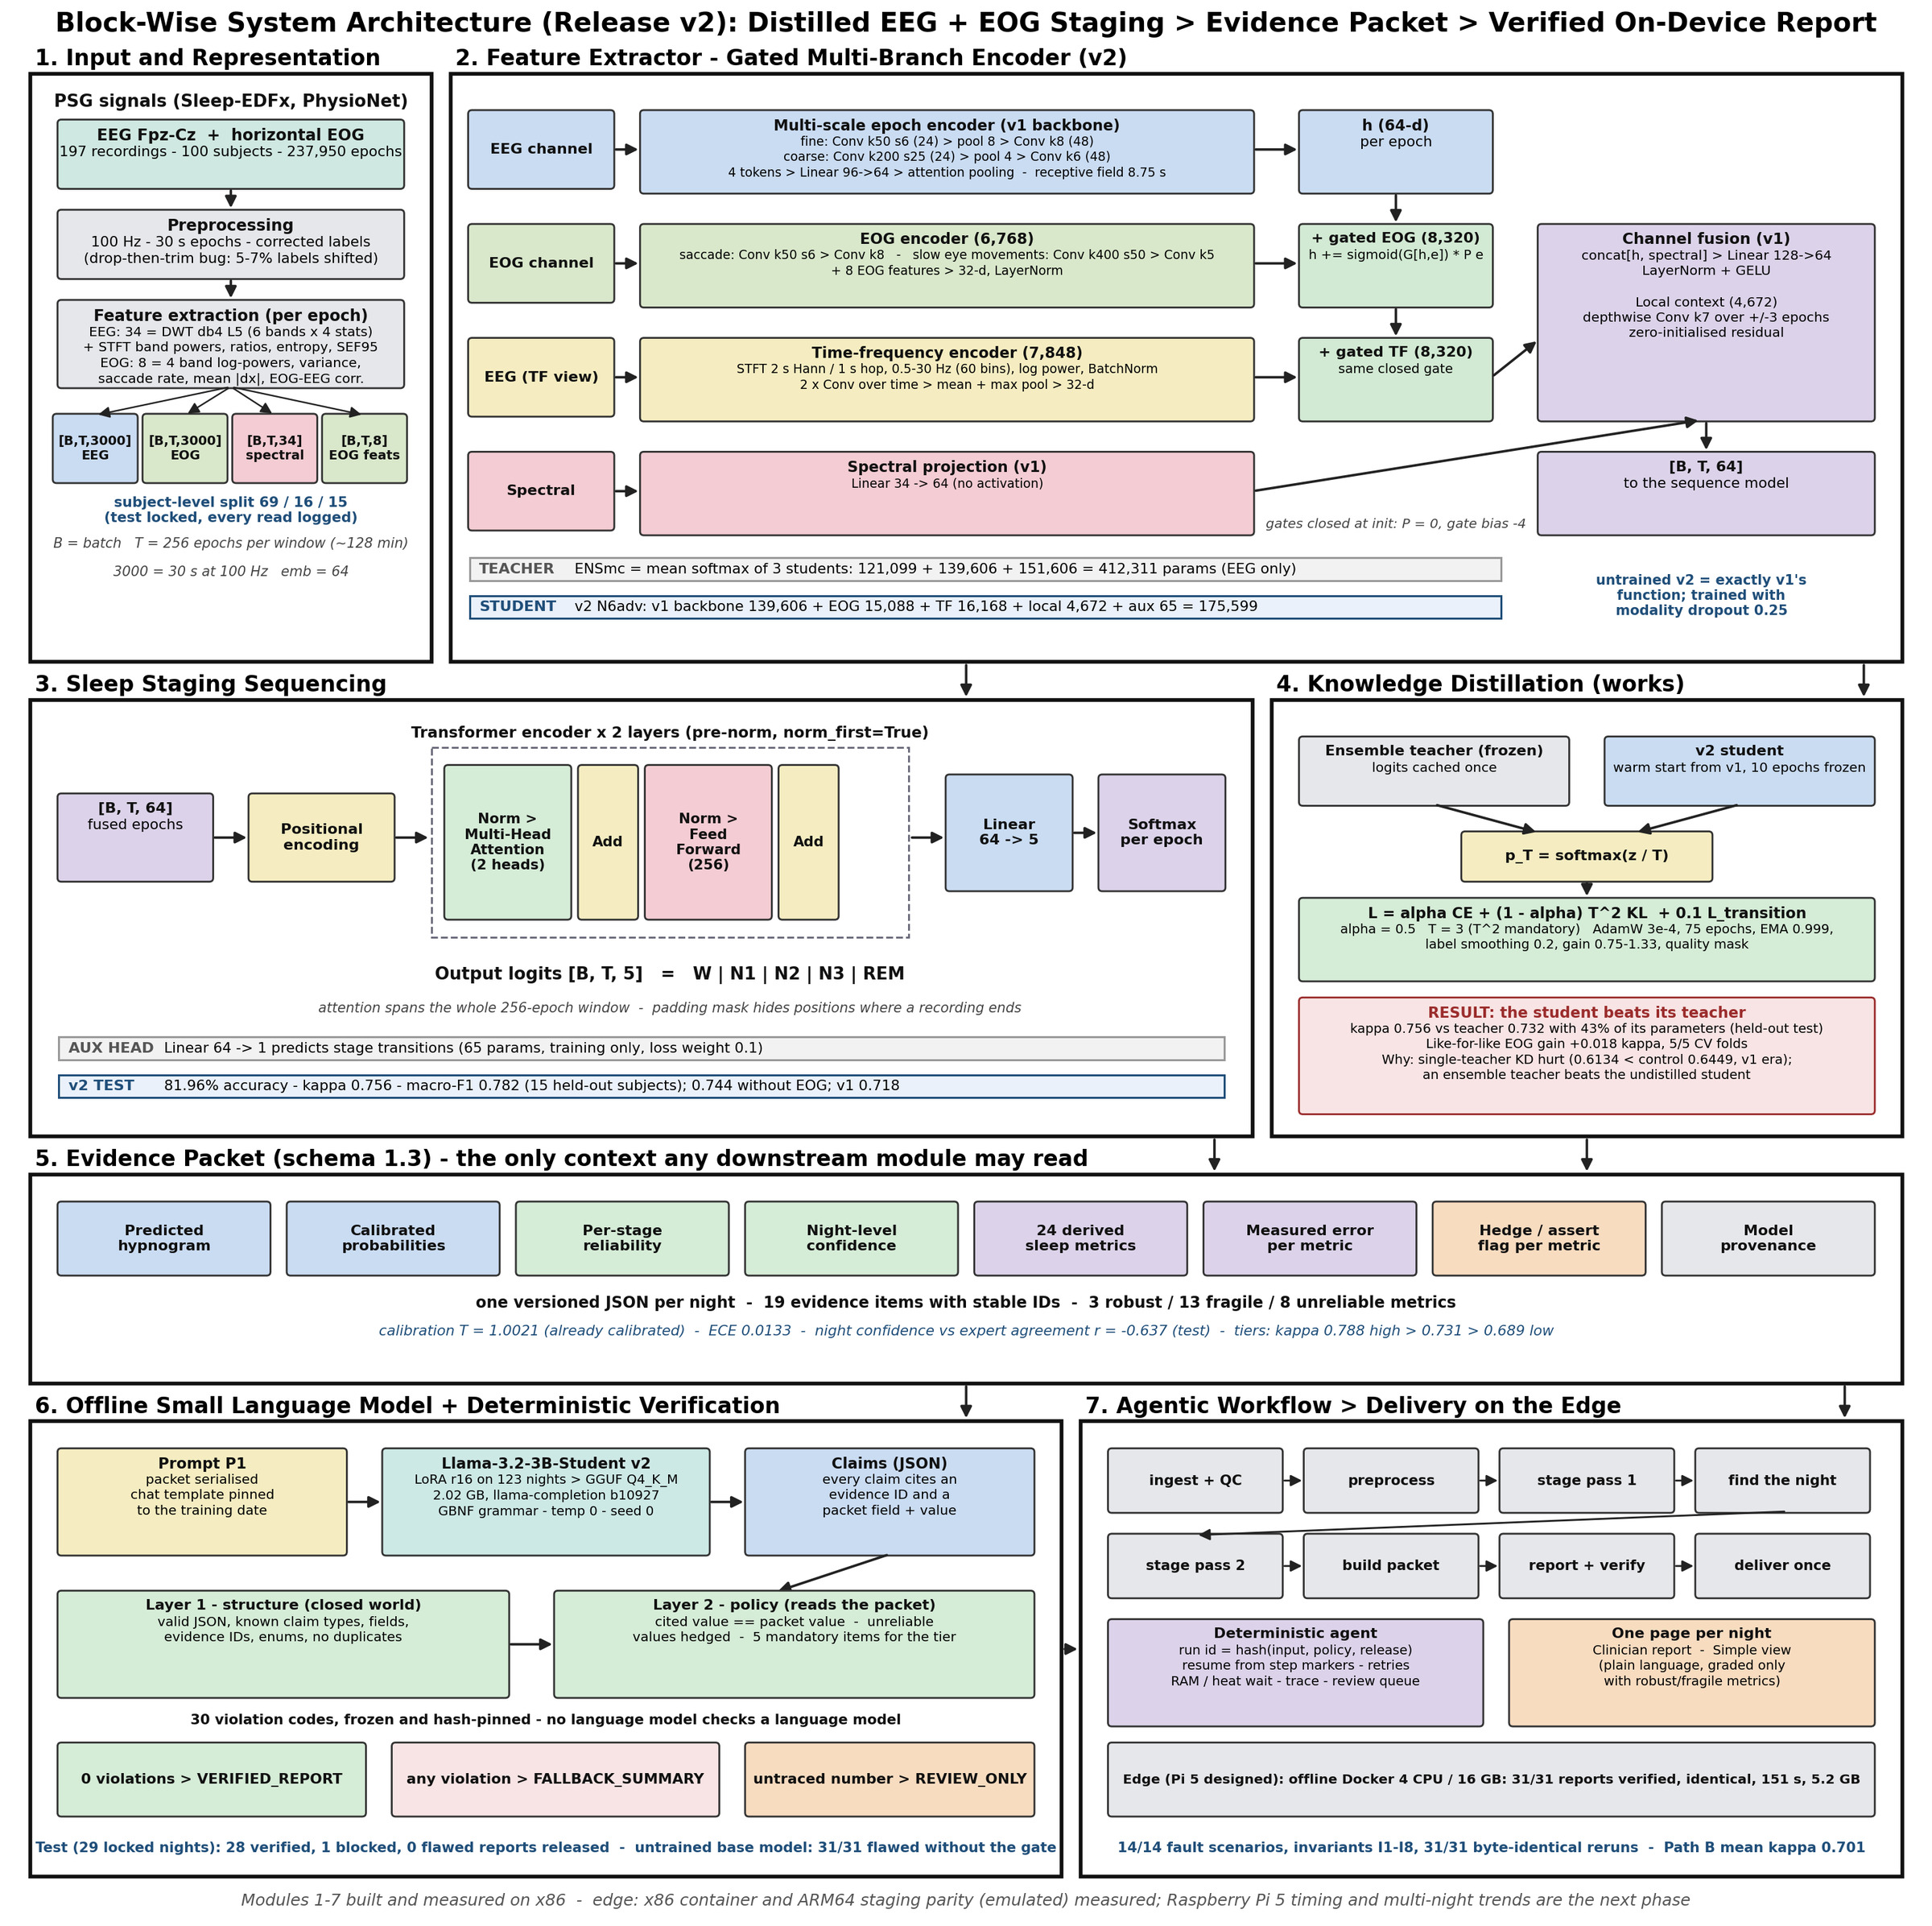
\includegraphics[width=\textwidth]{A0_blockwise_architecture_v2.jpg}
\caption{Block-wise architecture of release v2, with each block's measured result.}
\label{fig:blockwise}
\end{figure}

\textbf{Teacher.} The ensemble teacher ENSmc averages the softmax of three students of the same family
(121,099 + 139,606 + 151,606 = \textbf{412,311} parameters). It replaced a single 649,229-parameter teacher after
the experiments in Section~\ref{sec:res-kd}.

\textbf{Student, release v1 (N4kd, 139,606 parameters, historical).} One EEG channel plus 34 spectral features, read
as sequences of 256 epochs (about 2\,h). A multi-scale epoch encoder has a fine branch (Conv k50 s6, 24 channels
$\rightarrow$ max-pool 8 $\rightarrow$ Conv k8, 48) and a coarse branch (Conv k200 s25, 24 $\rightarrow$ max-pool 4
$\rightarrow$ Conv k6, 48); both are pooled to 4 tokens, projected 96$\rightarrow$64 and attention-pooled into a
64-d epoch vector. The spectral features are projected 34$\rightarrow$64, fused (Linear, LayerNorm, GELU), given
sinusoidal positions and passed through a 2-layer pre-norm Transformer encoder (d 64, 2 heads, FF 256) with a
5-class head. The encoder's measured receptive field is \textbf{8.75\,s}, wide enough to contain a spindle,
K-complex or slow wave; the original encoder's was 25 samples (0.25\,s) (Figure~\ref{fig:rf}).

\begin{figure}[htbp]
\centering
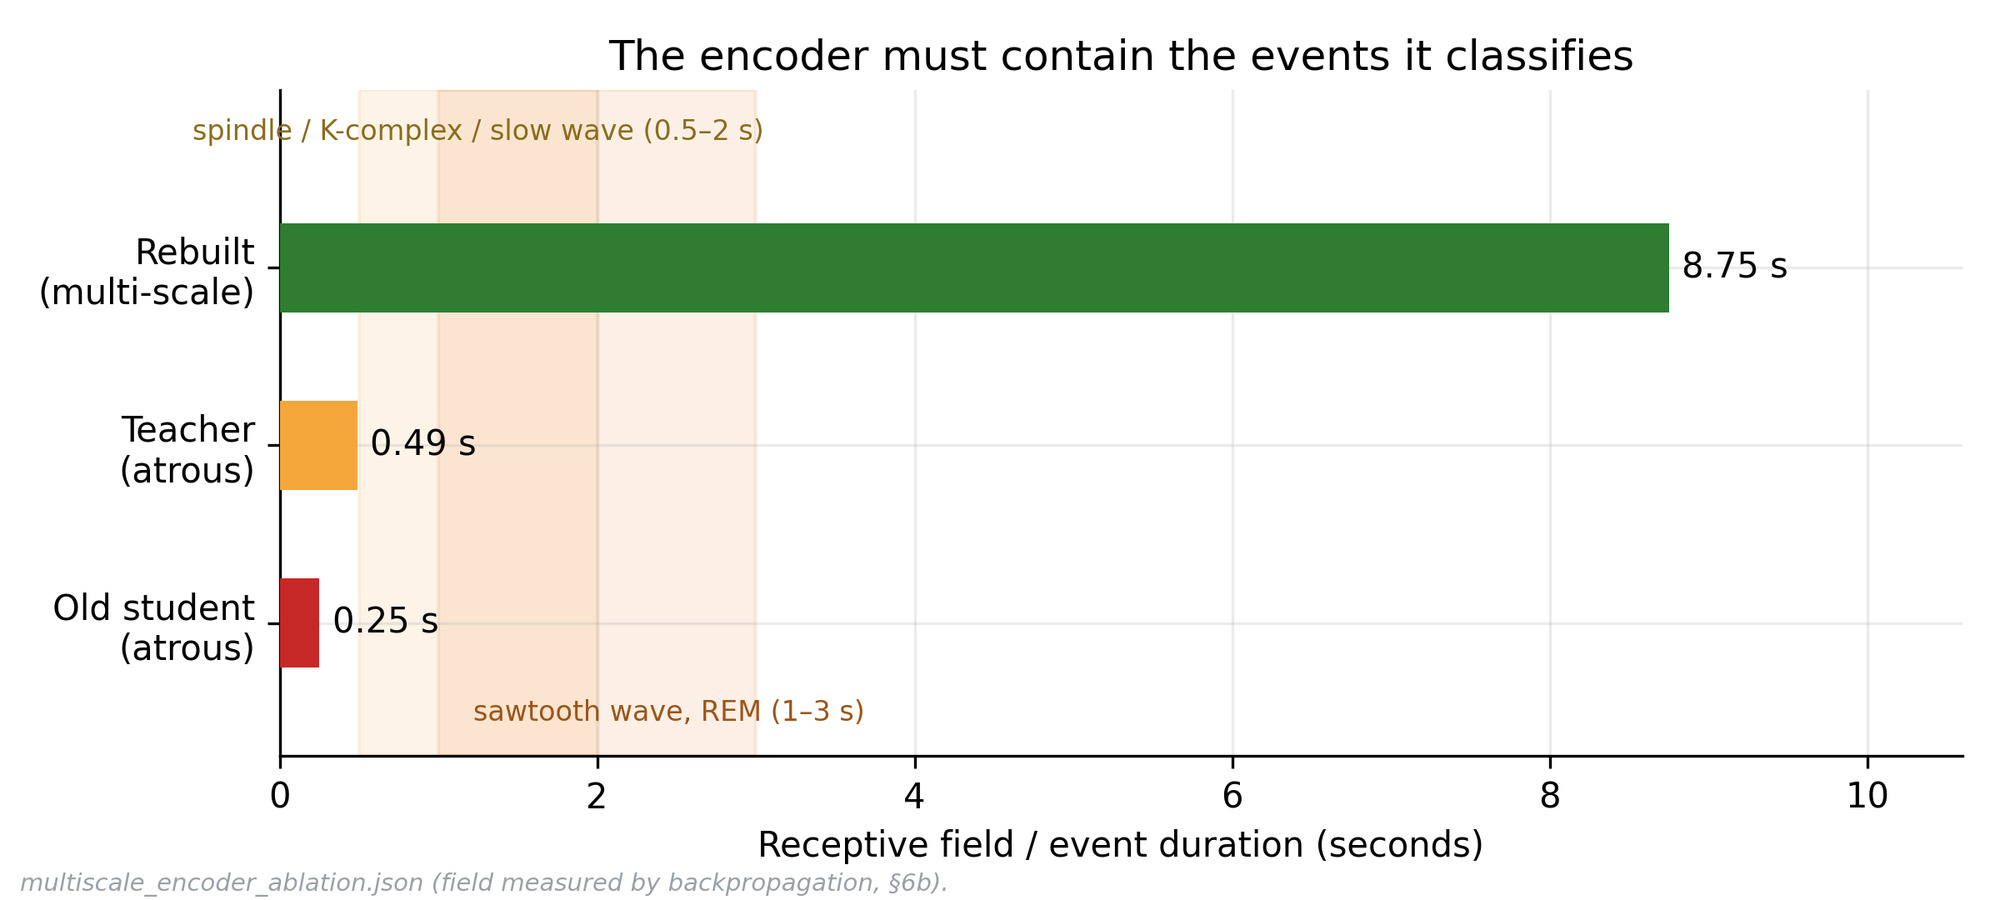
\includegraphics[width=0.8\textwidth]{v1_F5_receptive_field.jpg}
\caption{Measured receptive field of the original (0.25\,s) and multi-scale (8.75\,s) encoders.}
\label{fig:rf}
\end{figure}

\textbf{Student, release v2 (N6adv ``full'', 175,599 parameters, current).} The v1 backbone is kept unchanged and
three parts are added, each joining through a \textbf{gate that starts closed}: the projection is zero-initialised
and the gate bias is $-4$, so at initialisation the model computes exactly v1's function and moves away only where
that helps (Figure~\ref{fig:student}, Table~\ref{tab:params}). For an epoch representation $h$ and a branch output
$e$, each gated branch adds
\begin{equation}
h \leftarrow h + \sigma\!\left(W_g [h; e] + b_g\right) \odot P e, \qquad P = 0,\; b_g = -4 \text{ at initialisation.}
\end{equation}
The gated EOG and time-frequency residuals are added to $h$ in turn, then $h$ is fused with the spectral
projection, refined by a zero-initialised local-context convolution over $\pm3$ neighbouring epochs, and passed to
the Transformer.

\begin{figure}[htbp]
\centering
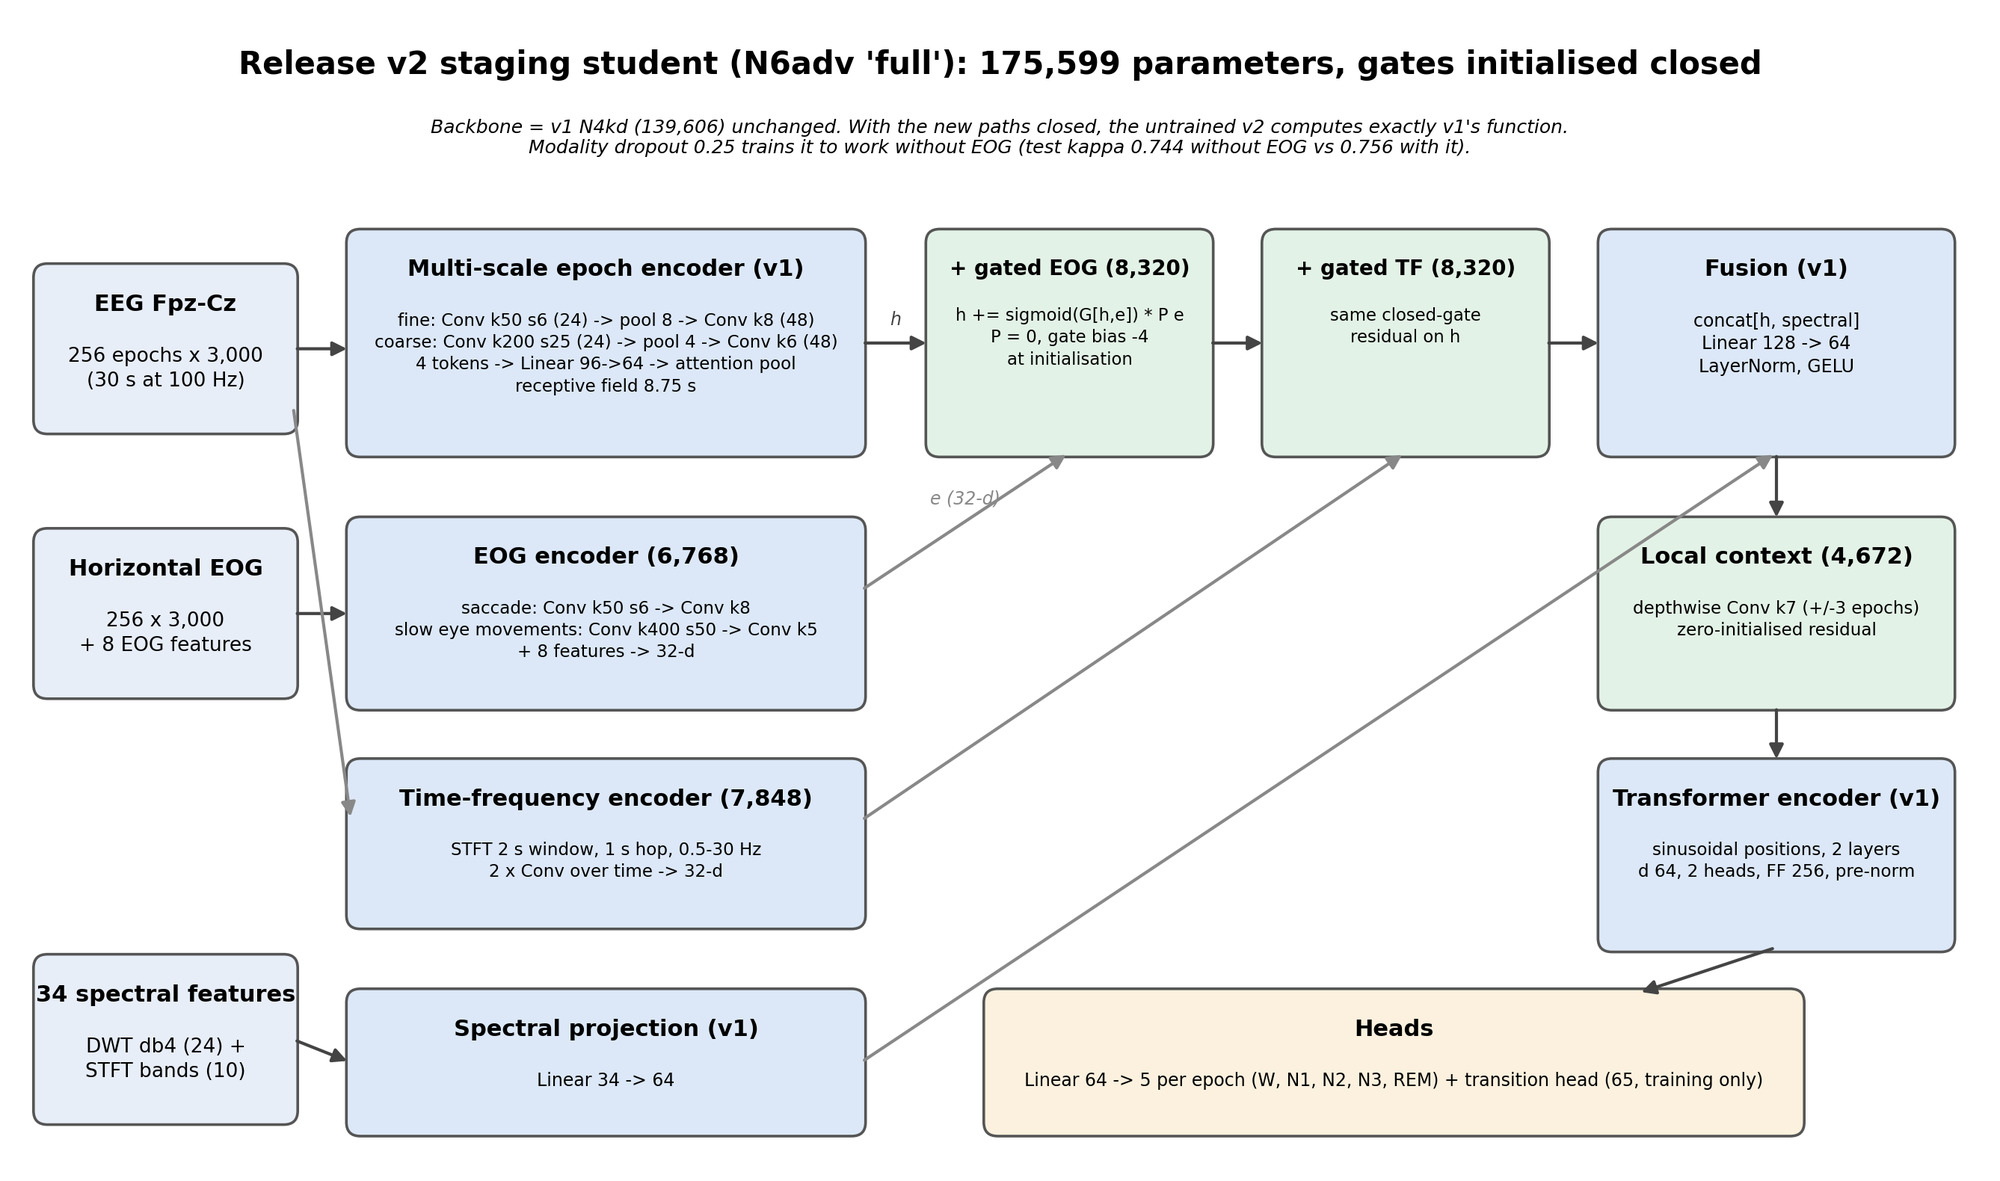
\includegraphics[width=\textwidth]{A2_staging_model_v2.jpg}
\caption{Architecture of the release v2 staging student (from \texttt{AdvancedStudent} in the training code).}
\label{fig:student}
\end{figure}

\begin{table}[htbp]
\centering\small
\caption{Release v2 staging student: parameter budget.}
\label{tab:params}
\begin{tabularx}{\textwidth}{lYr}
\toprule
Part & What it does & Params \\
\midrule
v1 backbone & Multi-scale encoder, spectral projection, fusion, Transformer, head (unchanged) & 139,606 \\
EOG encoder & Saccade branch (Conv k50 s6) + slow-eye-movement branch (Conv k400 s50) + 8 hand-made EOG features $\rightarrow$ 32-d & 6,768 \\
EOG projection + gate & 32 $\rightarrow$ 64, sigmoid gate on $[h, e]$ & 8,320 \\
Time-frequency encoder & STFT (2\,s window, 1\,s hop), 0.5--30\,Hz in 0.5\,Hz bins, 2 convolutions $\rightarrow$ 32-d & 7,848 \\
TF projection + gate & 32 $\rightarrow$ 64, sigmoid gate & 8,320 \\
Local context & Depthwise conv k7 over $\pm$3 epochs, zero-initialised & 4,672 \\
Auxiliary transition head & Predicts stage changes (training only) & 65 \\
\midrule
\textbf{Total} & & \textbf{175,599} \\
\bottomrule
\end{tabularx}
\end{table}

\textbf{Evidence packet.} A deterministic builder turns per-epoch probabilities into a versioned JSON packet
(Table~\ref{tab:packet}). Fields that are not yet populated are present and \texttt{null}, so adding them later
does not break consumers.

\begin{table}[htbp]
\centering\small
\caption{Evidence packet schema 1.3 (top-level fields).}
\label{tab:packet}
\begin{tabularx}{\textwidth}{lY}
\toprule
Field & Content \\
\midrule
\texttt{schema\_version} & "1.3"; consumers refuse a mismatch \\
\texttt{recording\_id}, \texttt{subject\_id}, \texttt{cohort} & Identity \\
\texttt{provenance} & Model, checkpoint sha256, git commit, calibration temperature, decoder, generator \\
\texttt{hypnogram}, \texttt{decoding} & Predicted stages, stage runs, how the hypnogram was decoded \\
\texttt{probabilities} & Calibrated per-epoch probabilities, 5 classes \\
\texttt{per\_stage} & Counts, mean confidence, model reliability tier per stage \\
\texttt{derived\_metrics} & 24 metrics (TST, efficiency, WASO, REM latency, \ldots) \\
\texttt{derived\_metric\_reliability} & Which metrics may be asserted: robust / fragile / unreliable, from measured error \\
\texttt{night\_confidence} & Tier and mean entropy; no ground truth needed \\
\texttt{evidence\_items} & 19 items with stable IDs that claims must cite \\
\texttt{attribution}, \texttt{risk} & Integrated-Gradients profile (v1 packets); risk reserved \\
\bottomrule
\end{tabularx}
\end{table}

\textbf{Report model and verifier (Figure~\ref{fig:verifier}).} Llama-3.2-3B-Instruct~\cite{llama32} with LoRA
adapters~\cite{hu2022lora}, quantised to Q4\_K\_M (2.02\,GB), is run by \texttt{llama-completion} (llama.cpp
b10927~\cite{llamacpp}) under a GBNF grammar that admits only the claim schema, at temperature 0 and seed 0, with a
chat template pinned to its training date. The verifier has two layers. Layer~1 (structure, packet-independent)
owns the closed world: valid JSON, known claim types, fields, evidence IDs and enums, no duplicates. Layer~2
(policy, reads the packet) checks that every cited value equals the packet's value exactly, that unreliable values
are hedged, that nothing is double-counted, that no unsafe item is cited without a review flag, and that the five
mandatory items for the night's tier are covered --- 30 violation codes in total. A rendered page passes a final
V-HTML check that every number on it traces to the packet.

\begin{figure}[htbp]
\centering
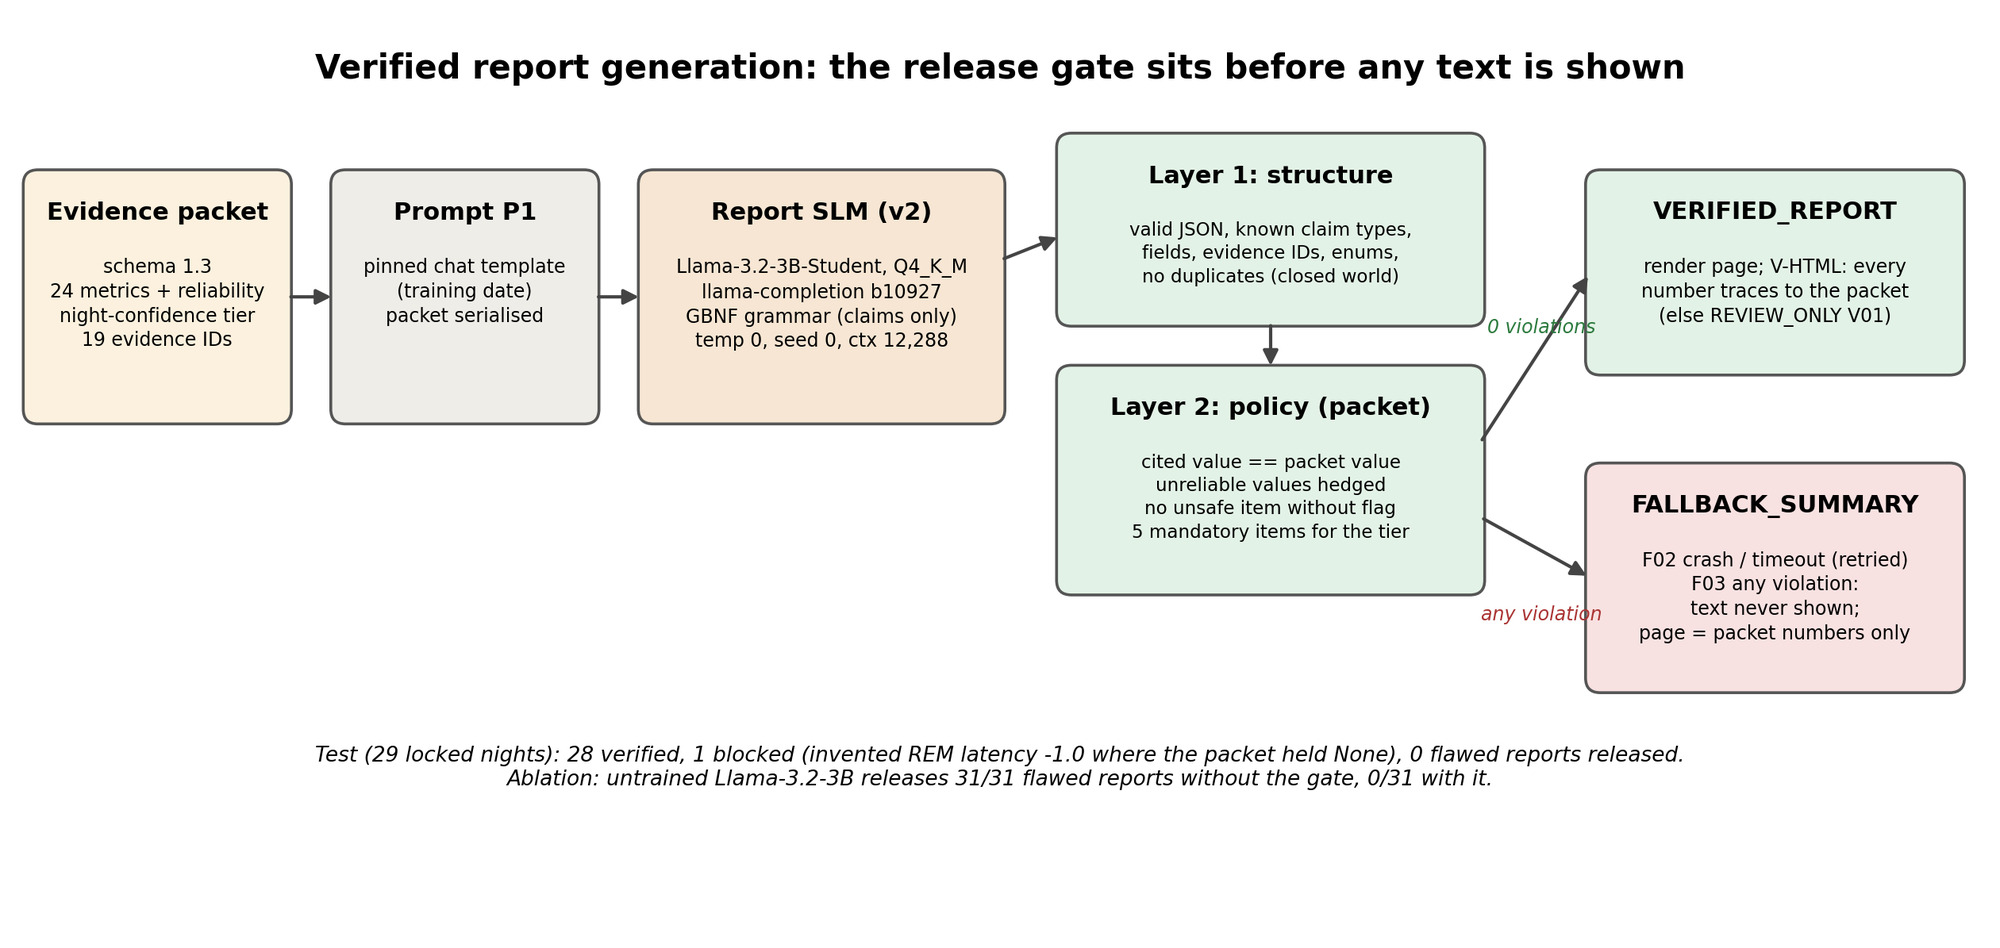
\includegraphics[width=\textwidth]{A3_report_and_verifier.jpg}
\caption{Verified report generation: the release gate sits before any text is shown.}
\label{fig:verifier}
\end{figure}

\textbf{Agent (Figure~\ref{fig:agent}).} A state machine whose steps each write to their own directory and return a
decision naming the next step. Run identity is a hash of the input, the policy and the release manifest. Finished
steps are replayed from their markers, an interrupted step is wiped and re-run, every transition is traced, and the
walk is bounded so a run always ends. Path~A starts from a prebuilt packet; Path~B starts from a raw EDF with no
expert hypnogram.

\begin{figure}[htbp]
\centering
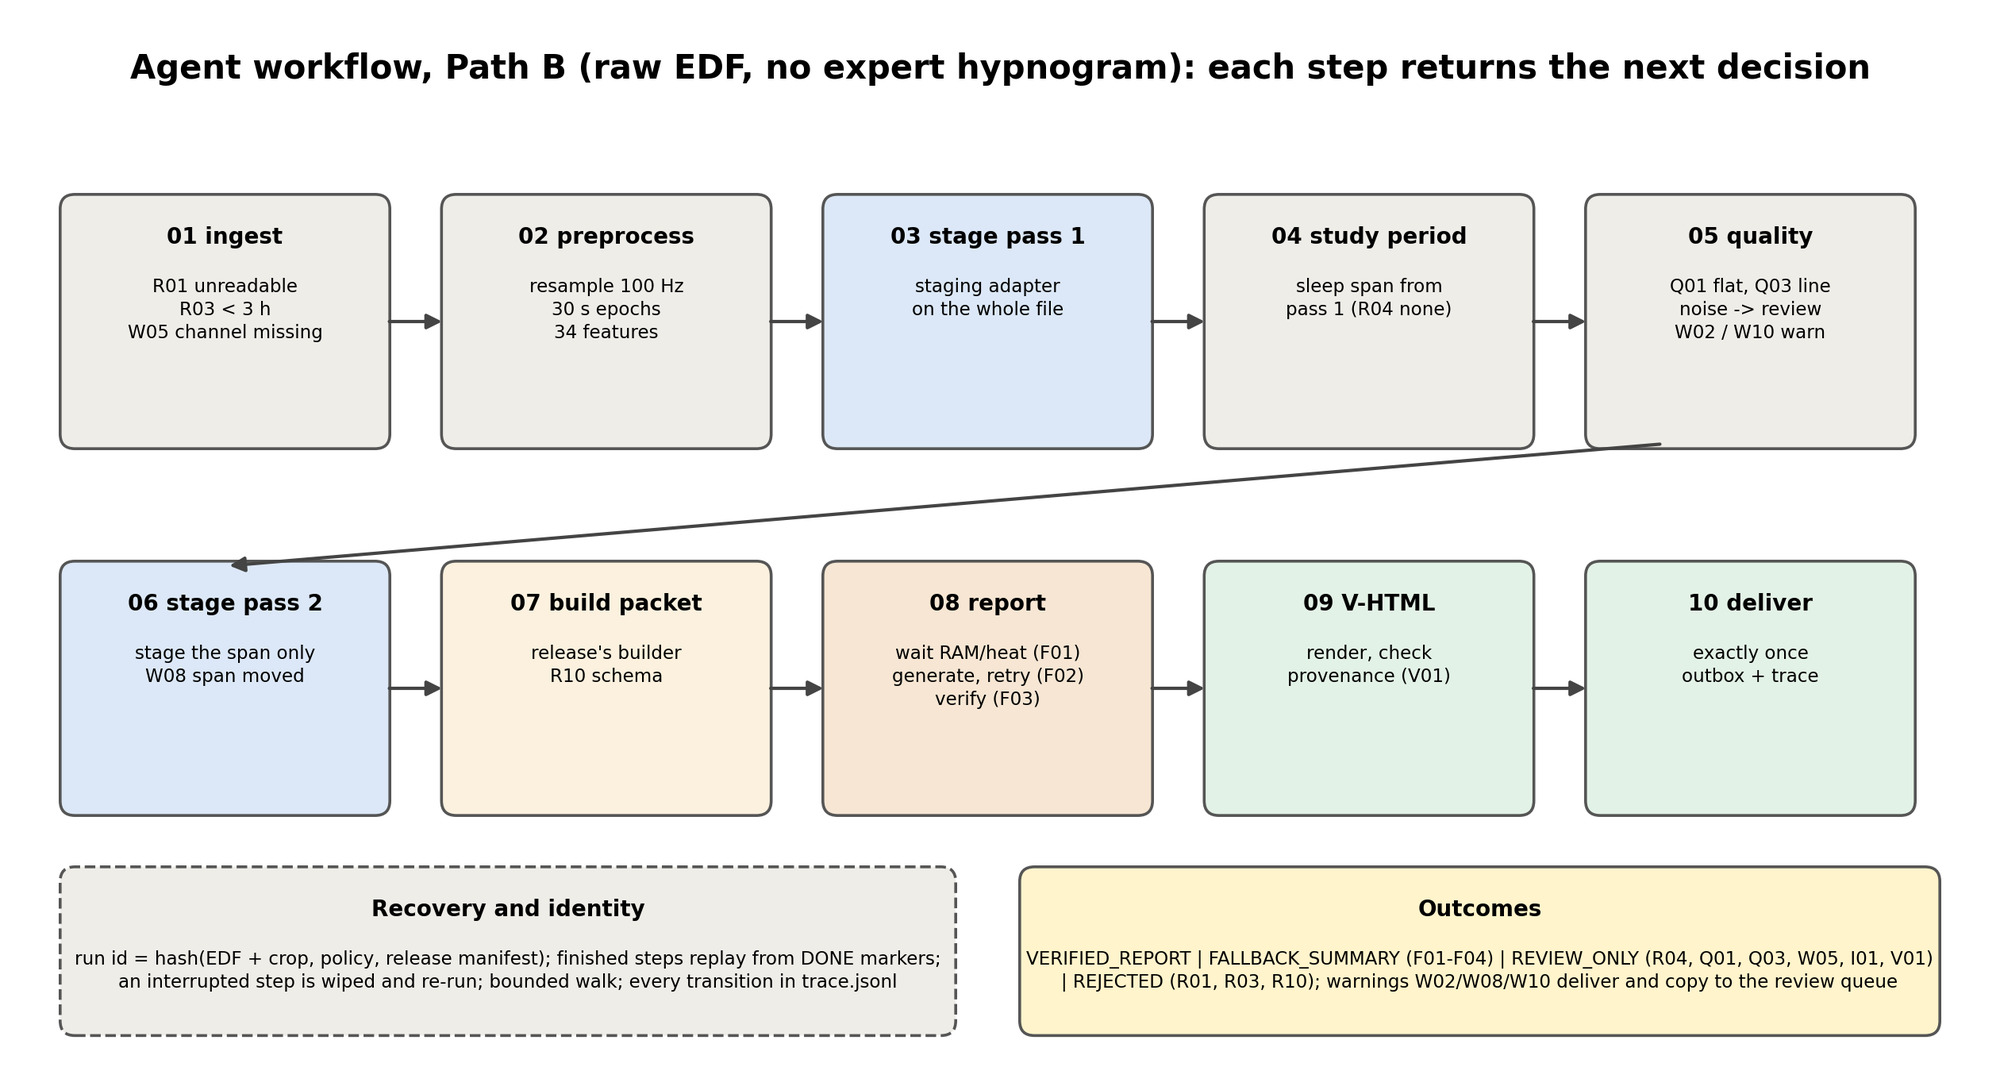
\includegraphics[width=\textwidth]{A4_agent_workflow.jpg}
\caption{Agent workflow, Path B: each step returns the next decision; reason codes name every exit.}
\label{fig:agent}
\end{figure}

\textbf{Plain-language layer.} A deterministic, template-based summary for non-experts grades the packet's values
against age-specific reference ranges. It shows only robust and fragile metrics in the main text (fragile ones
with "could be off by about X"), moves unreliable ones to "details for your doctor", always states what the test
cannot detect, and is checked by a self-test that every number traces to the packet or the reference table. It is
not written by the language model.

\subsection{Tools and Technologies:}

\begin{table}[htbp]
\centering\small
\caption{Tools and technologies.}
\label{tab:tools}
\begin{tabularx}{\textwidth}{lY}
\toprule
Area & Tools \\
\midrule
Language & Python 3 \\
Signal processing & MNE (EDF reading, resampling), PyWavelets (DWT), SciPy (STFT, Welch for EOG), NumPy, pandas \\
Staging models & PyTorch; trained on Kaggle (NVIDIA T4) \\
Report model & Hugging Face Transformers + PEFT (LoRA) on Kaggle T4; llama.cpp b10927 for GGUF Q4\_K\_M inference on CPU \\
Reference model & Gemini 3.1 Flash, used once offline to establish the contract and generate training targets \\
Constrained decoding & GBNF grammar \\
Agent & Plain-Python state machine, YAML release manifests and policy, sha256 pinning, atomic file writes \\
Interface & FastAPI + Uvicorn local console (\texttt{python -m ui}), static HTML/JS, no external assets \\
Testing & pytest (agent, KD loss, splits, provenance), fault injection \\
Edge & Docker (CPU and memory limits, \texttt{--network none}), QEMU/buildx for ARM64; Raspberry Pi 5 (designed) \\
\bottomrule
\end{tabularx}
\end{table}

\subsection{Algorithm or Model Description}

\textbf{Knowledge-distillation loss.} For student logits $z_s$, teacher logits $z_t$, labels $y$, mixing weight
$\alpha$ and temperature $T$:
\begin{equation}
\mathcal{L} = \alpha\,\mathrm{CE}(z_s, y) + (1-\alpha)\,T^2\,\mathrm{KL}\!\left(\mathrm{softmax}(z_t/T)\,\Vert\,\mathrm{softmax}(z_s/T)\right),
\end{equation}
with $\alpha = 0.5$ and $T = 3$. The $T^2$ factor keeps the soft-target gradient on the same scale as the hard-label
gradient; without it training still runs but silently learns worse, so a unit test covers it. Teacher outputs are
cached once rather than recomputed every epoch.

\begin{algorithm}[htbp]
\caption{Ensemble-teacher distillation of the staging student}\label{alg:kd}
\begin{algorithmic}[1]
\State \textbf{Input} subject-disjoint training recordings $R$; trained students $S_1 \ldots S_K$; architecture $A$; $\alpha$, $T$
\State \textbf{Output} distilled student $S^*$
\For{each recording $r \in R$}
  \State $z_t[r] \gets \log\!\big(\tfrac{1}{K}\sum_k \mathrm{softmax}(S_k(r))\big)$ \Comment{ensemble teacher, cached}
\EndFor
\State initialise $S^*$ from $A$ (warm start from the v1 backbone; new gates closed)
\For{epoch $= 1 \ldots 75$}
  \For{each batch of 256-epoch sequences $(x, y, r)$}
    \State $\mathcal{L} \gets \alpha\,\mathrm{CE}(S^*(x), y) + (1-\alpha)\,T^2\,\mathrm{KL}(\mathrm{softmax}(z_t[r]/T) \Vert \mathrm{softmax}(S^*(x)/T))$
    \State $\mathcal{L} \gets \mathcal{L} + 0.1 \cdot$ transition loss \Comment{auxiliary head}
    \State update $S^*$ with AdamW; update EMA weights
  \EndFor
  \State keep $S^*$ if validation macro-F1 improves \Comment{validation only, never test}
\EndFor
\end{algorithmic}
\end{algorithm}

Training details (v2): warm start from v1 with the backbone frozen for 10 epochs, then trained at 0.1$\times$
learning rate; AdamW (lr $3\times10^{-4}$, weight decay $10^{-2}$); boundary-aware label smoothing ($\varepsilon$
0.2); a quality mask that leaves flat or stuck epochs out of the loss; amplitude augmentation (0.75--1.33$\times$)
with the spectral features moved consistently; EMA (0.999); modality dropout 0.25, so EOG and TF are each switched
off for a quarter of training sequences and the model learns to cope without them; three seeds.

\textbf{Calibration and confidence.} Temperature scaling fits one scalar $T_c$ on validation by minimising negative
log-likelihood and applies it unchanged to test. Night confidence is the mean prediction entropy over the night;
tier boundaries are validation-entropy tertiles.

\textbf{Derived-metric reliability.} For each of the 24 metrics, the error between the value computed from
predicted stages and from expert stages is measured on validation, and the metric is classed robust, fragile or
unreliable. The report may assert only robust values plainly; the others must be hedged.

\begin{algorithm}[htbp]
\caption{Verified report generation for one night (Path A)}\label{alg:report}
\begin{algorithmic}[1]
\State \textbf{Input} evidence packet $P$, release manifest $M$, policy $\Pi$
\State \textbf{Output} exactly one delivered page
\If{sha256 of model, grammar, template, verifier or renderer $\neq M$.pinned} \Return REVIEW\_ONLY (I01) \EndIf
\State prompt $\gets$ build\_prompt(P1, $P$)
\State wait until free RAM and temperature satisfy $\Pi$; on timeout \Return FALLBACK (F01)
\For{attempt $= 1 \ldots 1 + \Pi$.retries}
  \State text $\gets$ llama-completion(model, prompt, grammar, temp $=0$, seed $=0$)
  \If{process succeeded and end marker seen} \textbf{break} \EndIf
\EndFor
\If{generation failed} \Return FALLBACK (F02) \EndIf
\State $V \gets$ verify\_structure(text) $\cup$ verify\_policy(text, $P$)
\If{$V \neq \emptyset$} \Return FALLBACK (F03) \Comment{text is never rendered} \EndIf
\State page $\gets$ render(text, $P$); \textbf{if} refused \textbf{return} FALLBACK (F04)
\If{page contains a number without packet provenance} \Return REVIEW\_ONLY (V01) \EndIf
\State deliver page to the outbox exactly once; log the run
\end{algorithmic}
\end{algorithm}

\begin{algorithm}[htbp]
\caption{Agentic Path B: raw EDF, no expert hypnogram}\label{alg:pathb}
\begin{algorithmic}[1]
\State \textbf{ingest:} reject if unreadable (R01) or shorter than 3\,h (R03); review if a required channel is missing (W05)
\State \textbf{preprocess:} resample to 100\,Hz; 30-s epochs; 34 spectral features
\State \textbf{stage pass 1:} staging adapter on the whole file
\State \textbf{study period:} estimate the sleep span from pass-1 stages; review if none (R04)
\State \textbf{quality:} flat / stuck / line-noise fraction; review above threshold (Q01, Q03), warn otherwise (W02, W10)
\State \textbf{stage pass 2:} stage only the span; warn if the span moved (W08)
\State \textbf{build packet:} the release's own packet builder; reject on schema mismatch (R10)
\State \textbf{report:} Algorithm~\ref{alg:report}; annotate the page with a quality note; V-HTML check; deliver
\end{algorithmic}
\end{algorithm}

\begin{table}[htbp]
\centering\small
\caption{Agent outcomes and reason codes.}
\label{tab:outcomes}
\begin{tabularx}{\textwidth}{lYY}
\toprule
Outcome & When & Examples \\
\midrule
VERIFIED\_REPORT & Every claim passed the verifier and the page passed V-HTML & -- \\
FALLBACK\_SUMMARY & A report could not be produced safely; the page shows packet numbers only & F01 heat / low RAM, F02 crash / timeout, F03 verifier violations, F04 render refused \\
REVIEW\_ONLY & The night cannot be summarised safely; nothing is shown & R04 no sleep span, Q01/Q03 bad signal, W05 missing channel, I01 changed hashes, V01 untraced number \\
REJECTED & Input fails minimum requirements & R01 unreadable, R03 too short, R10 schema mismatch \\
\bottomrule
\multicolumn{3}{l}{\footnotesize Warnings (W02, W08, W10) still deliver a report but copy the run to the review queue.}
\end{tabularx}
\end{table}

\textbf{Edge budget model.} Token generation for a quantised model on a CPU is limited by memory bandwidth: each
generated token reads all weights once, so
\begin{equation}
\text{tokens/s} \approx \frac{\text{effective memory bandwidth}}{\text{bytes read per token}}.
\end{equation}
For Llama-3.2-3B Q4\_K\_M this gives a ceiling of 7.43 tokens/s at the Pi 5's theoretical 17\,GB/s, and 3.06--4.37
tokens/s at an assumed effective 7--10\,GB/s. Figure~\ref{fig:edge} shows the target device and the simulation
ladder used to validate it step by step.

\begin{figure}[htbp]
\centering
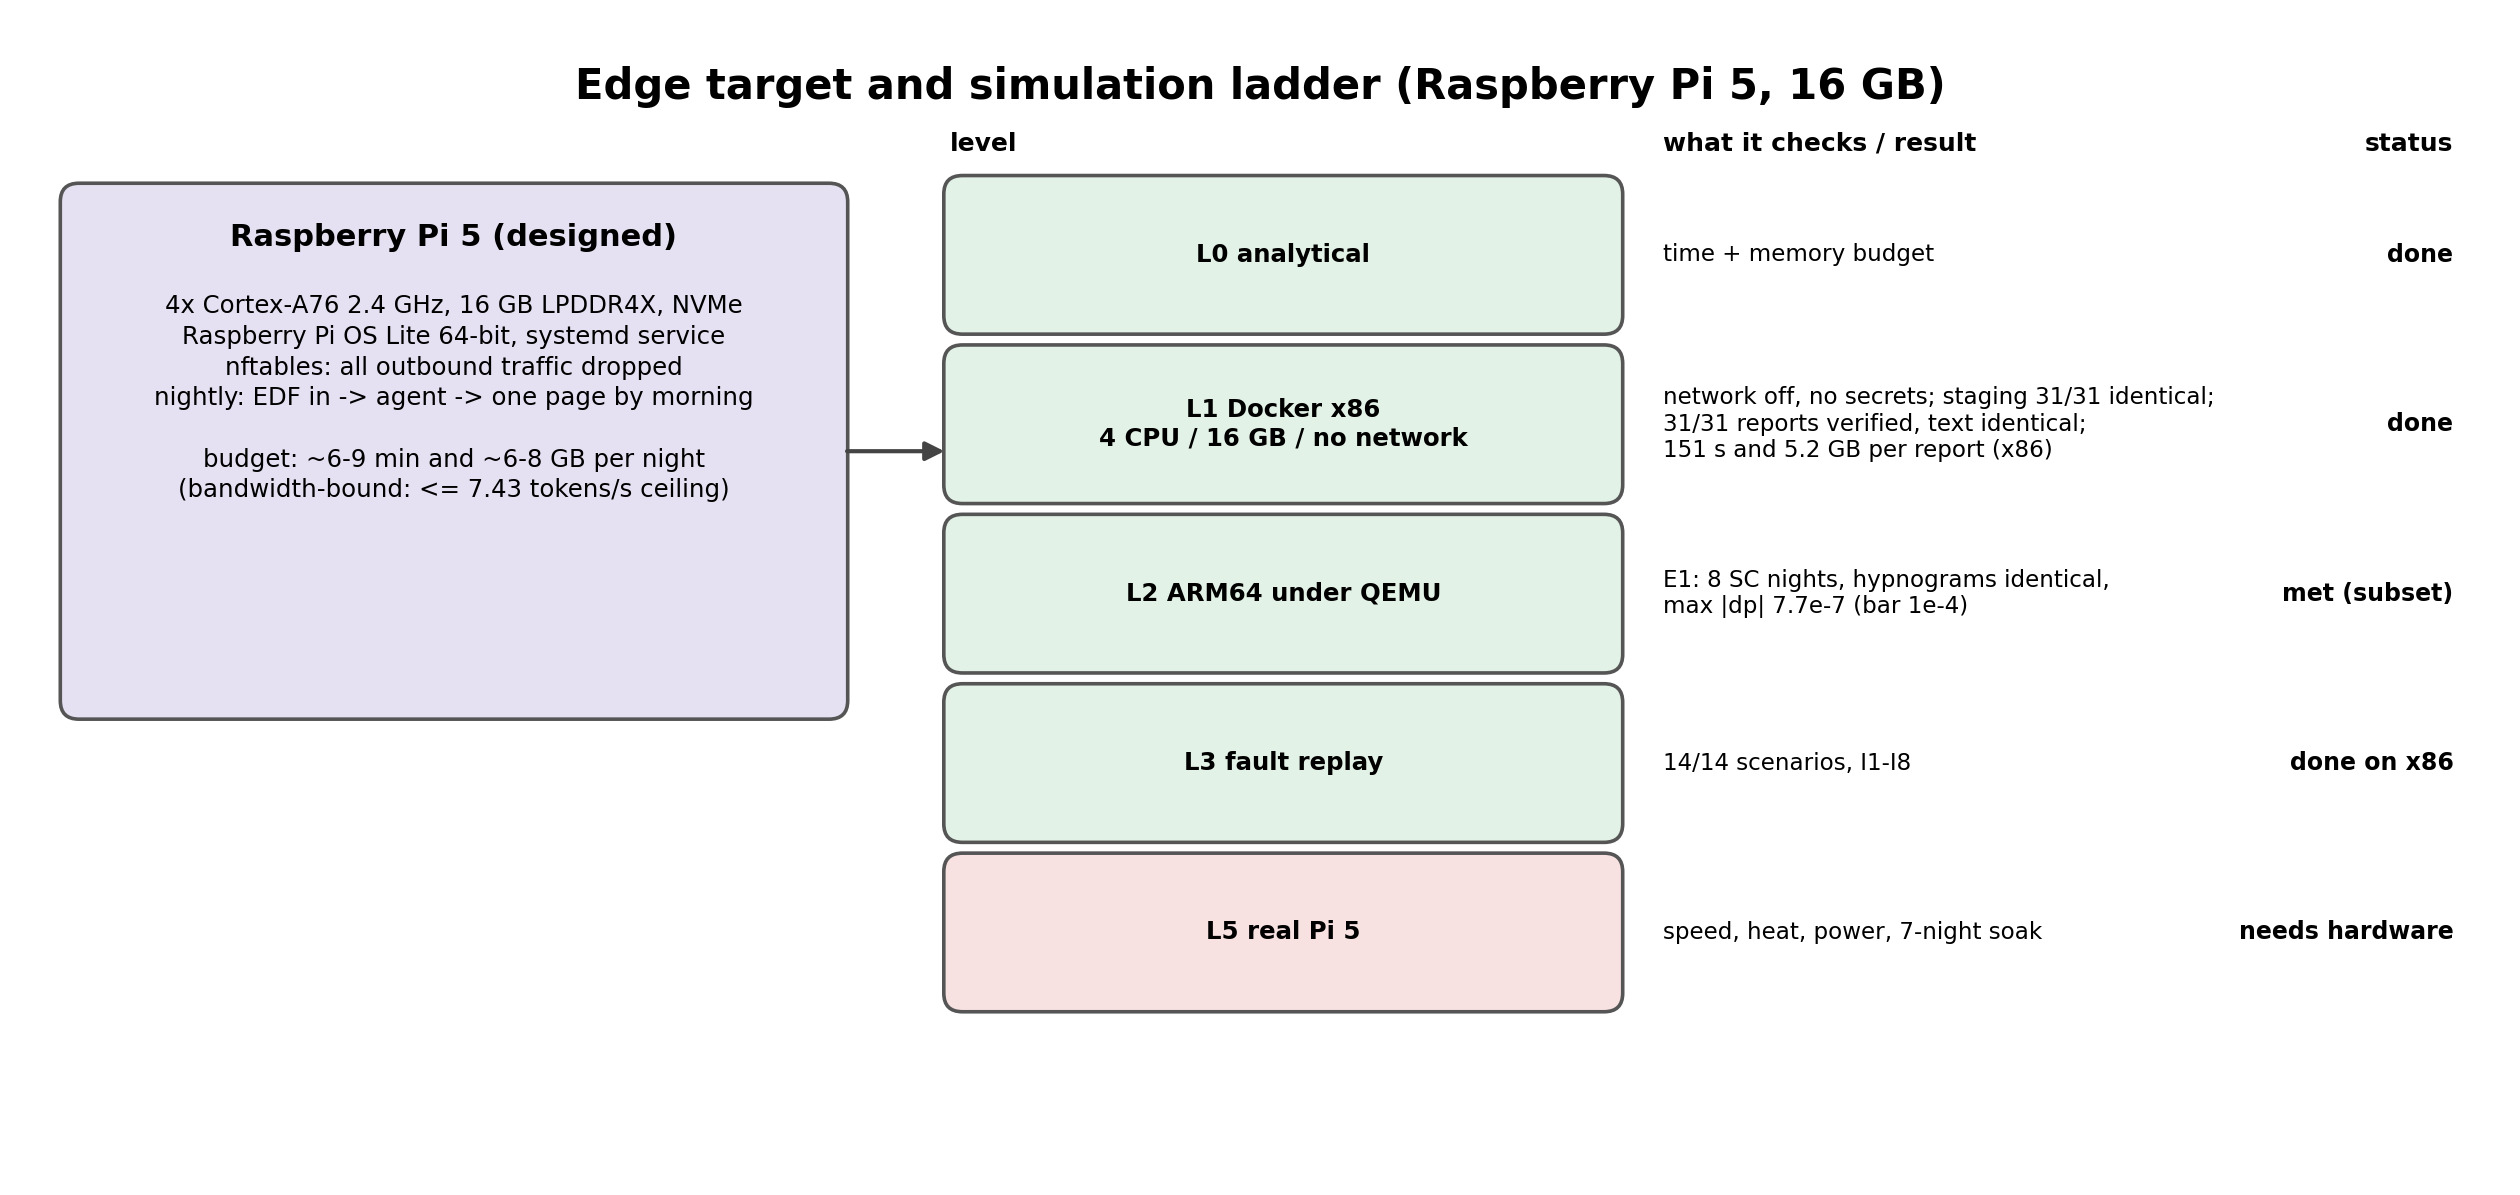
\includegraphics[width=\textwidth]{A6_edge_and_simulation.jpg}
\caption{Edge target (Raspberry Pi 5) and the simulation ladder with its current status.}
\label{fig:edge}
\end{figure}

\subsection{ Expected Outcomes}

\begin{itemize}
  \item A staging student under 200\,K parameters at or above its teacher's $\kappa$ on unseen subjects, and
  competitive on the standard benchmark.
  \item An evidence packet whose confidence signals separate good nights from bad without ground truth.
  \item A report model that, behind the verifier, releases no flawed report on held-out nights.
  \item An agent that reaches the expected outcome in every fault scenario and reproduces its outputs exactly.
  \item An edge plan that holds up in emulation: offline, secret-free, and numerically identical across platforms.
\end{itemize}

\subsection{Advantages of the Proposed Work}

\begin{itemize}
  \item \textbf{Small.} The staging model is 0.70\,MB (fp32), smaller than every published model at its accuracy
  level except LightSleepX.
  \item \textbf{Safe by construction.} The verifier compares values exactly, so a released report cannot contain a
  number that differs from the packet; a failure produces a fallback, not a wrong report.
  \item \textbf{Honest about uncertainty.} Each derived value carries its measured reliability; only 3 of 24 metrics
  are safe to state without qualification, and the report says so.
  \item \textbf{Private.} Everything runs offline; the container test confirmed no network is reachable.
  \item \textbf{Reproducible and auditable.} Every component is hash-pinned, runs are deterministic, and every run
  is traced.
  \item \textbf{Robust.} Missing EOG costs only 0.012 $\kappa$; bad signals, crashes, overheating and power loss each
  end in a defined, truthful outcome.
  \item \textbf{Swappable.} A new staging or report model is a new release file, not new agent code.
\end{itemize}

\subsection{Limitations and Assumptions}

\begin{itemize}
  \item \textbf{One dataset.} Everything rests on Sleep-EDFx. Within it, crossing from the SC to the ST cohort cost
  0.187 $\kappa$ for a v1-era model, which shows how little a single-dataset figure should be trusted to transfer.
  \item \textbf{Small evaluation sets.} 29 test nights give a 95\% lower bound of 82.2\% on 28/29. The test set has
  been read 7 times across the model line (logged, never for selection) and cannot evaluate any later model.
  \item \textbf{"Verified" means consistent with the packet}, not clinically correct. No clinician has rated a
  report, and the plain-language wording has not been tested with readers.
  \item \textbf{Label differences.} Corrected labels may differ from other papers' pipelines.
  \item \textbf{Night window.} Path~B uses the dataset's lights-off times for the device-like crop; the study-period
  end-point p90 error is 41 epochs on v2 against a 30-epoch bar (an accepted deviation). On some SC nights the
  research packets start before an evening nap, which inflates WASO; such nights are left ungraded in the
  plain-language view.
  \item \textbf{Edge numbers.} The Pi budget is analytical. Measured so far: an x86 container (timing on a desktop CPU,
  not the Pi's) and ARM64 staging parity under emulation on 8 Sleep Cassette nights. Not measured: the report model on
  ARM, Sleep Telemetry nights on ARM, and any timing, heat or power on a real Raspberry Pi 5.
  \item \textbf{The full system is not small.} The report model is 99.9\% of the footprint (2.02\,GB on disk, about
  4.7\,GB peak RAM).
\end{itemize}
